\chapter{Anexos técnicos}
\label{ch:anexos}

Este anexo resume el funcionamiento de la herramienta de visualización desarrollada para el proyecto. La aplicación, implementada en \acrshort{Streamlit}, centraliza resultados, facilita la comparación entre arquitecturas y mejora la interpretación cualitativa de las detecciones. El código completo se encuentra en \thegitrepo{}.

\section{Aportación principal de la herramienta}
\label{sec:anexo_aportacion}

La herramienta aporta valor en tres dimensiones:
\begin{itemize}
    \item \textbf{Reproducibilidad}: concentra metadatos y métricas de todos los experimentos.
    \item \textbf{Interpretabilidad}: permite contrastar \textit{ground truth} y predicciones por arquitectura.
    \item \textbf{Robustez}: integra análisis de score threshold para validar estabilidad del mejor modelo.
\end{itemize}

De este modo, la memoria no depende solo de tablas estáticas, sino también de un entorno interactivo para auditoría técnica.

\section{Funcionamiento técnico (resumen)}
\label{sec:anexo_funcionamiento}

\subsection{Entradas de datos}

La aplicación consume artefactos ya generados en el proyecto:
\begin{itemize}
    \item \texttt{experiments\_metadata.json} para inventario de experimentos.
    \item \texttt{test\_evaluation\_results*.json} para mAP, AP, precisión y recall.
    \item Resultados de \texttt{threshold\_analysis} para umbrales estrictos.
    \item Predicciones JSON y anotaciones COCO para visualización comparativa.
\end{itemize}

\subsection{Vistas disponibles}

La interfaz se organiza en seis vistas accesibles desde la barra lateral: \textbf{Inicio}, \textbf{Línea temporal}, \textbf{Explorador}, \textbf{Comparativa}, \textbf{Visualizaciones} y \textbf{Conclusiones}. Su propósito operativo es el siguiente:
\begin{itemize}
    \item \textbf{Inicio}: estado global del proyecto y métricas sintéticas para una lectura rápida.
    \item \textbf{Línea temporal}: recorrido cronológico de los experimentos y evolución del trabajo.
    \item \textbf{Explorador}: inspección de un experimento concreto (configuración, mejor checkpoint, mAP y métricas por clase).
    \item \textbf{Comparativa}: contraste entre arquitecturas con varios modos de análisis (\textit{todos}, \textit{mejores por arquitectura} y \textit{1024x1024}).
    \item \textbf{Visualizaciones}: validación cualitativa imagen a imagen, comparando \textit{ground truth} frente a predicción con \textit{score threshold} dinámico.
    \item \textbf{Conclusiones}: síntesis final para apoyar la toma de decisiones técnicas.
\end{itemize}

\section{Guía de uso breve}
\label{sec:anexo_guia_breve}

La herramienta está pensada como apoyo de auditoría técnica y se usa de forma iterativa: primero se selecciona el nivel de análisis (global, por experimento o por imagen) y después se ajustan filtros para confirmar hipótesis.

\begin{enumerate}
    \item Abrir la aplicación y elegir en la barra lateral la vista de trabajo.
    \item En \textbf{Explorador}, seleccionar un experimento para revisar su configuración, mAP@0.5 y comportamiento por clase (AP, precisión o recall).
    \item Si existe análisis de robustez, cambiar el \textit{score threshold} (0.15/0.75/0.90) para comprobar estabilidad de métricas.
    \item En \textbf{Comparativa}, activar opcionalmente la inclusión de thresholds altos y escoger el tipo de comparación más adecuado al objetivo.
    \item En \textbf{Visualizaciones}, seleccionar arquitectura, mover el \textit{slider} de threshold y navegar imágenes con los controles \textit{Anterior/Siguiente}.
    \item Contrastar siempre el resultado cuantitativo con la evidencia visual (\textit{ground truth} vs predicción) antes de extraer conclusiones.
\end{enumerate}

\textbf{Recomendación de uso:} no interpretar el mAP de forma aislada; combinarlo con precisión/recall por clase y con ejemplos visuales para detectar sesgos o falsos positivos relevantes.

\section{Capturas de la herramienta de visualización}
\label{sec:anexo_capturas_minimas}

Para no sobrecargar la memoria, se incluyen solo cuatro capturas clave que cubren el flujo principal de análisis de la aplicación.

\begin{figure}[htbp]
\centering
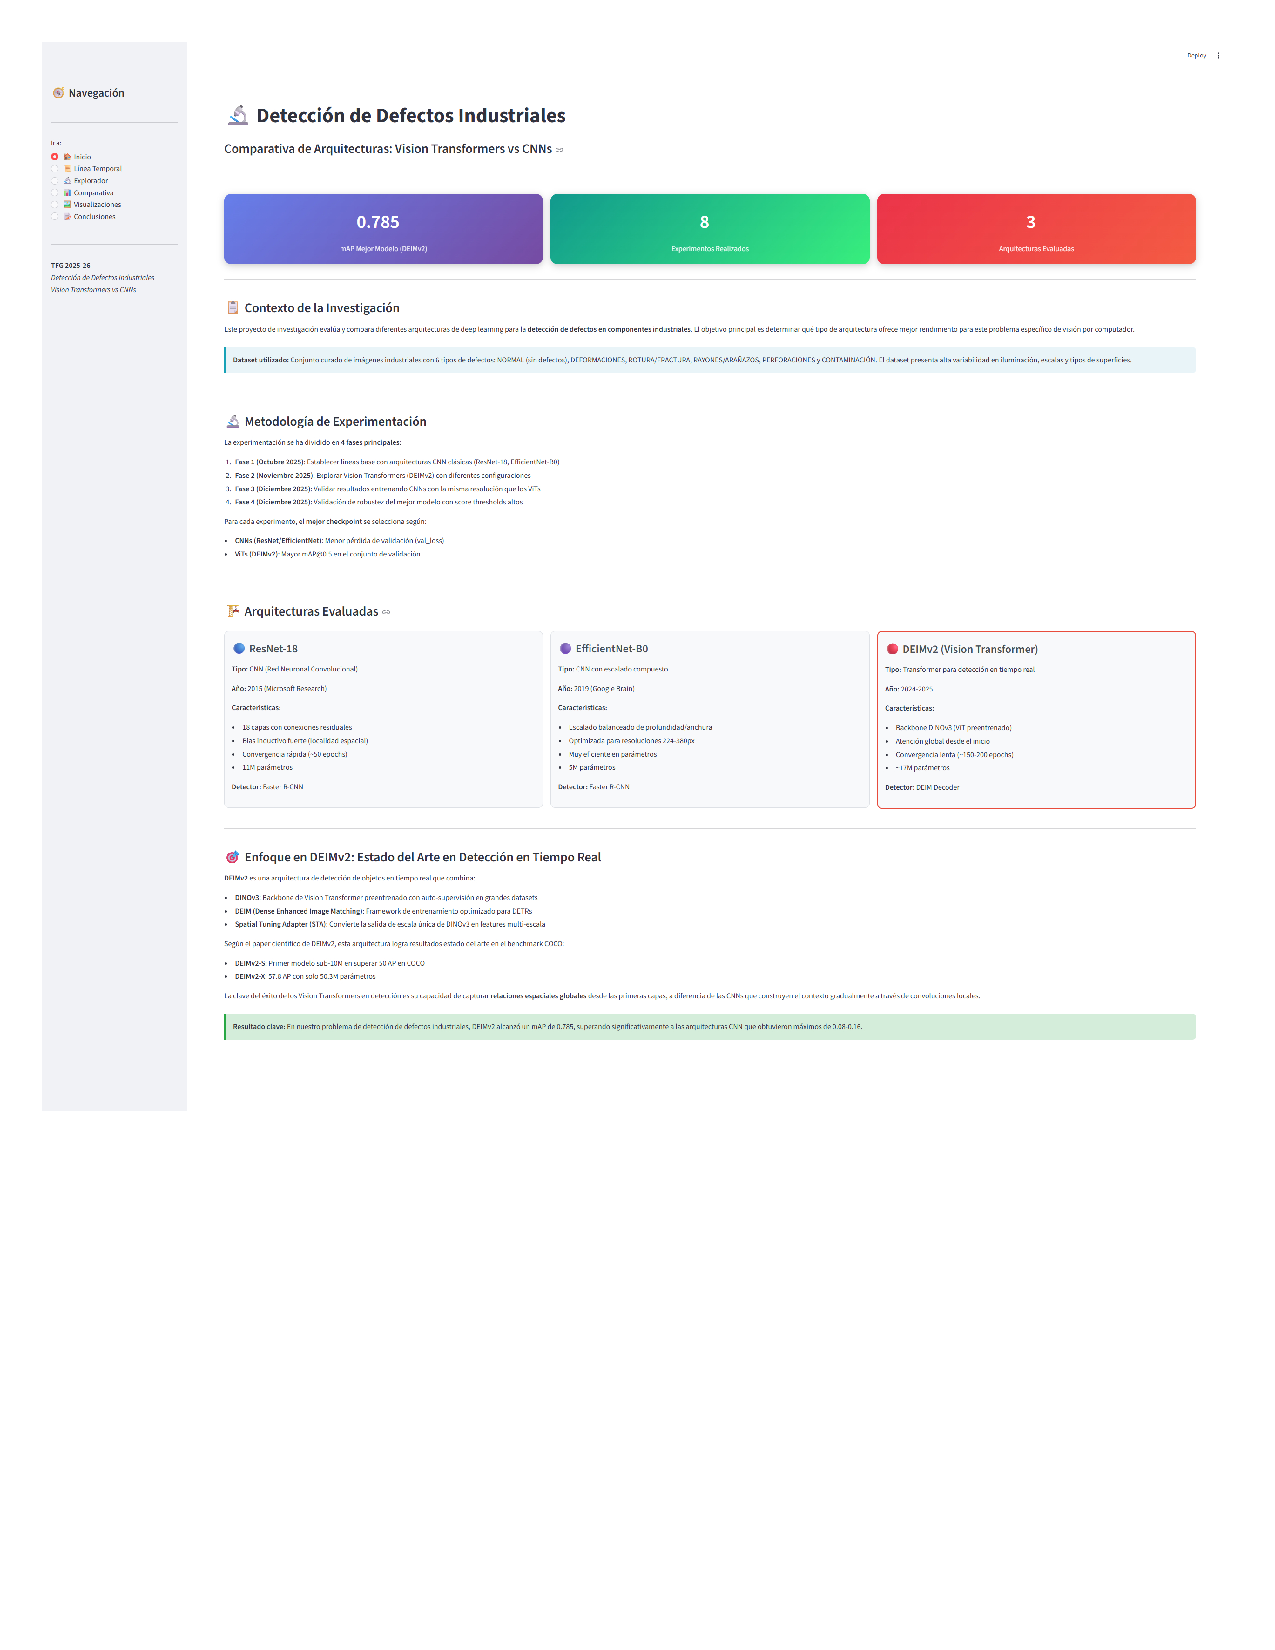
\includegraphics[width=0.95\textwidth]{fig/capturas-pantalla-herramienta-visualizacion/captura-vista-inicio.pdf}
\caption{Vista Inicio con resumen global de métricas y acceso a las secciones principales de análisis.}
\label{fig:anexo_cap_inicio}
\end{figure}

\begin{figure}[htbp]
\centering
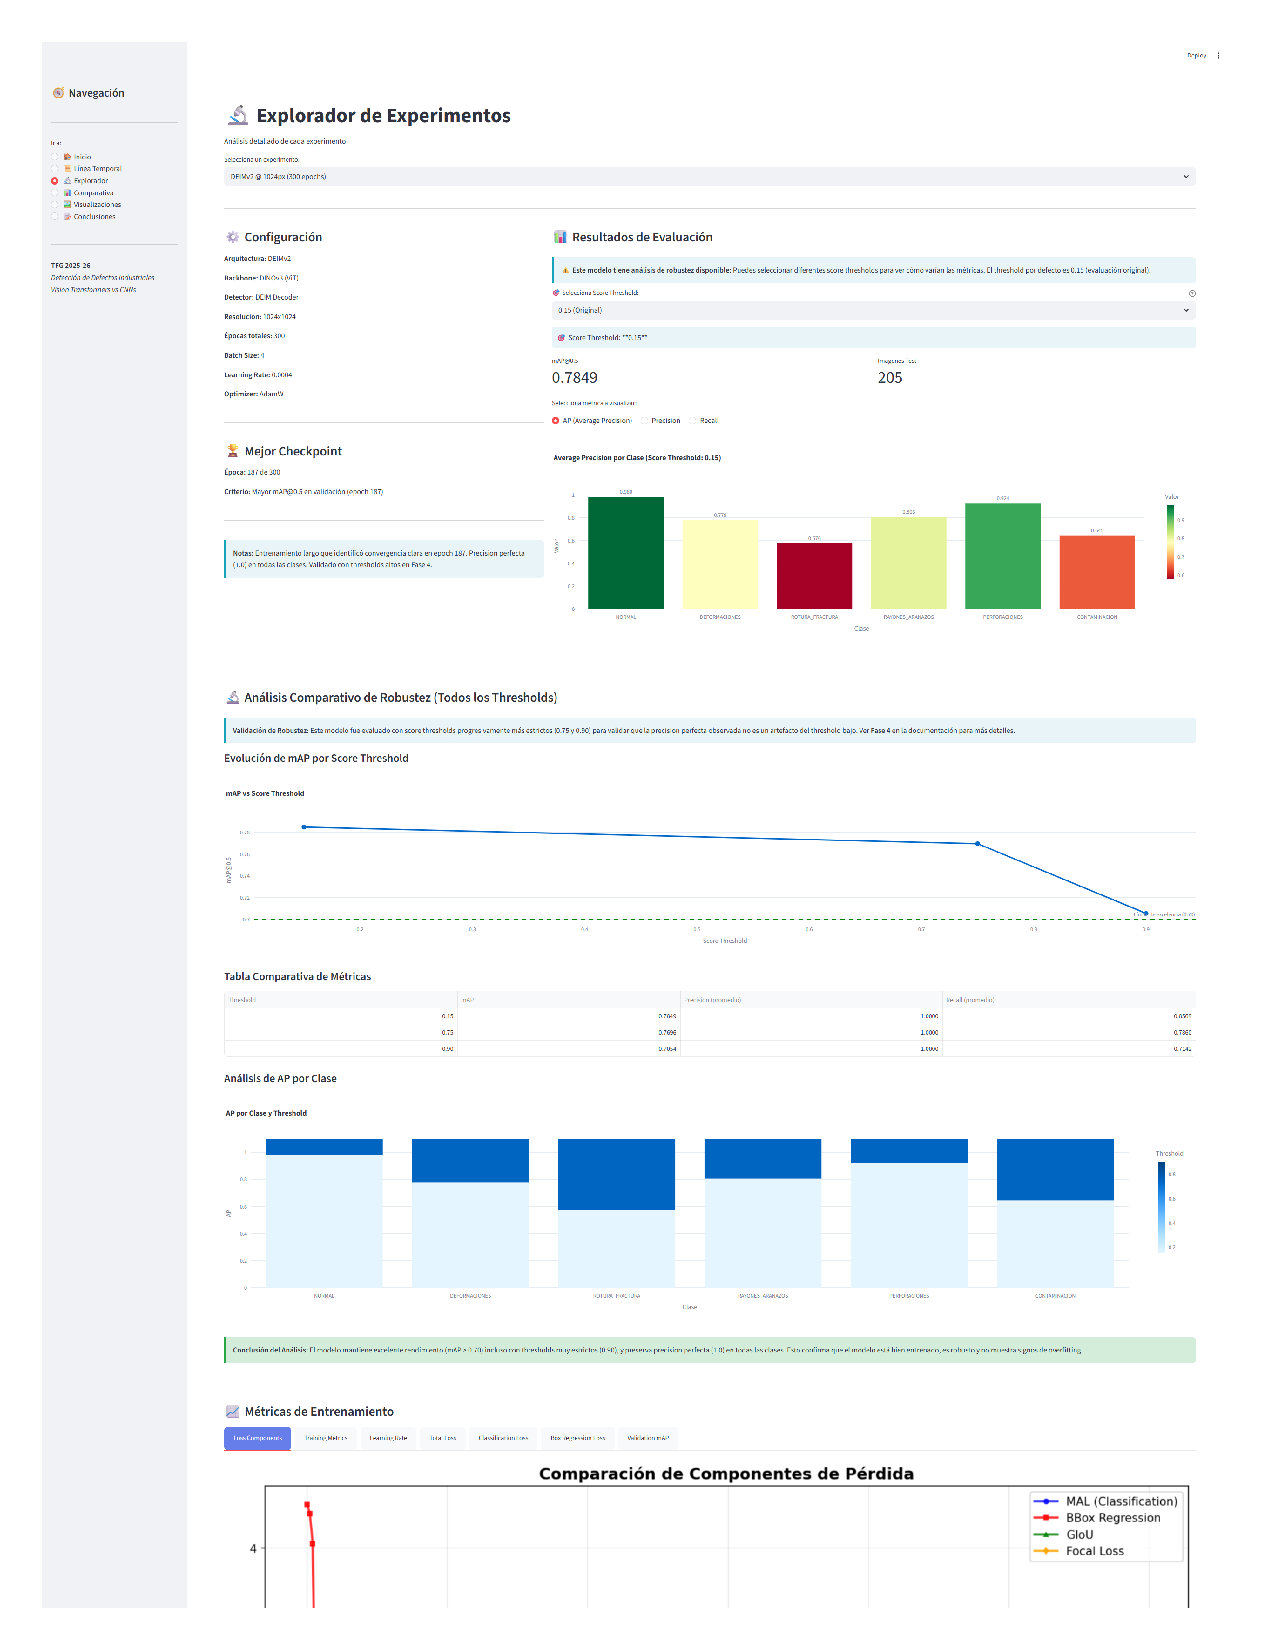
\includegraphics[width=0.95\textwidth]{fig/capturas-pantalla-herramienta-visualizacion/captura-vista-explorador.pdf}
\caption{Vista Explorador con detalle de un experimento, incluyendo configuración y métricas por clase.}
\label{fig:anexo_cap_explorador}
\end{figure}

\begin{figure}[htbp]
\centering
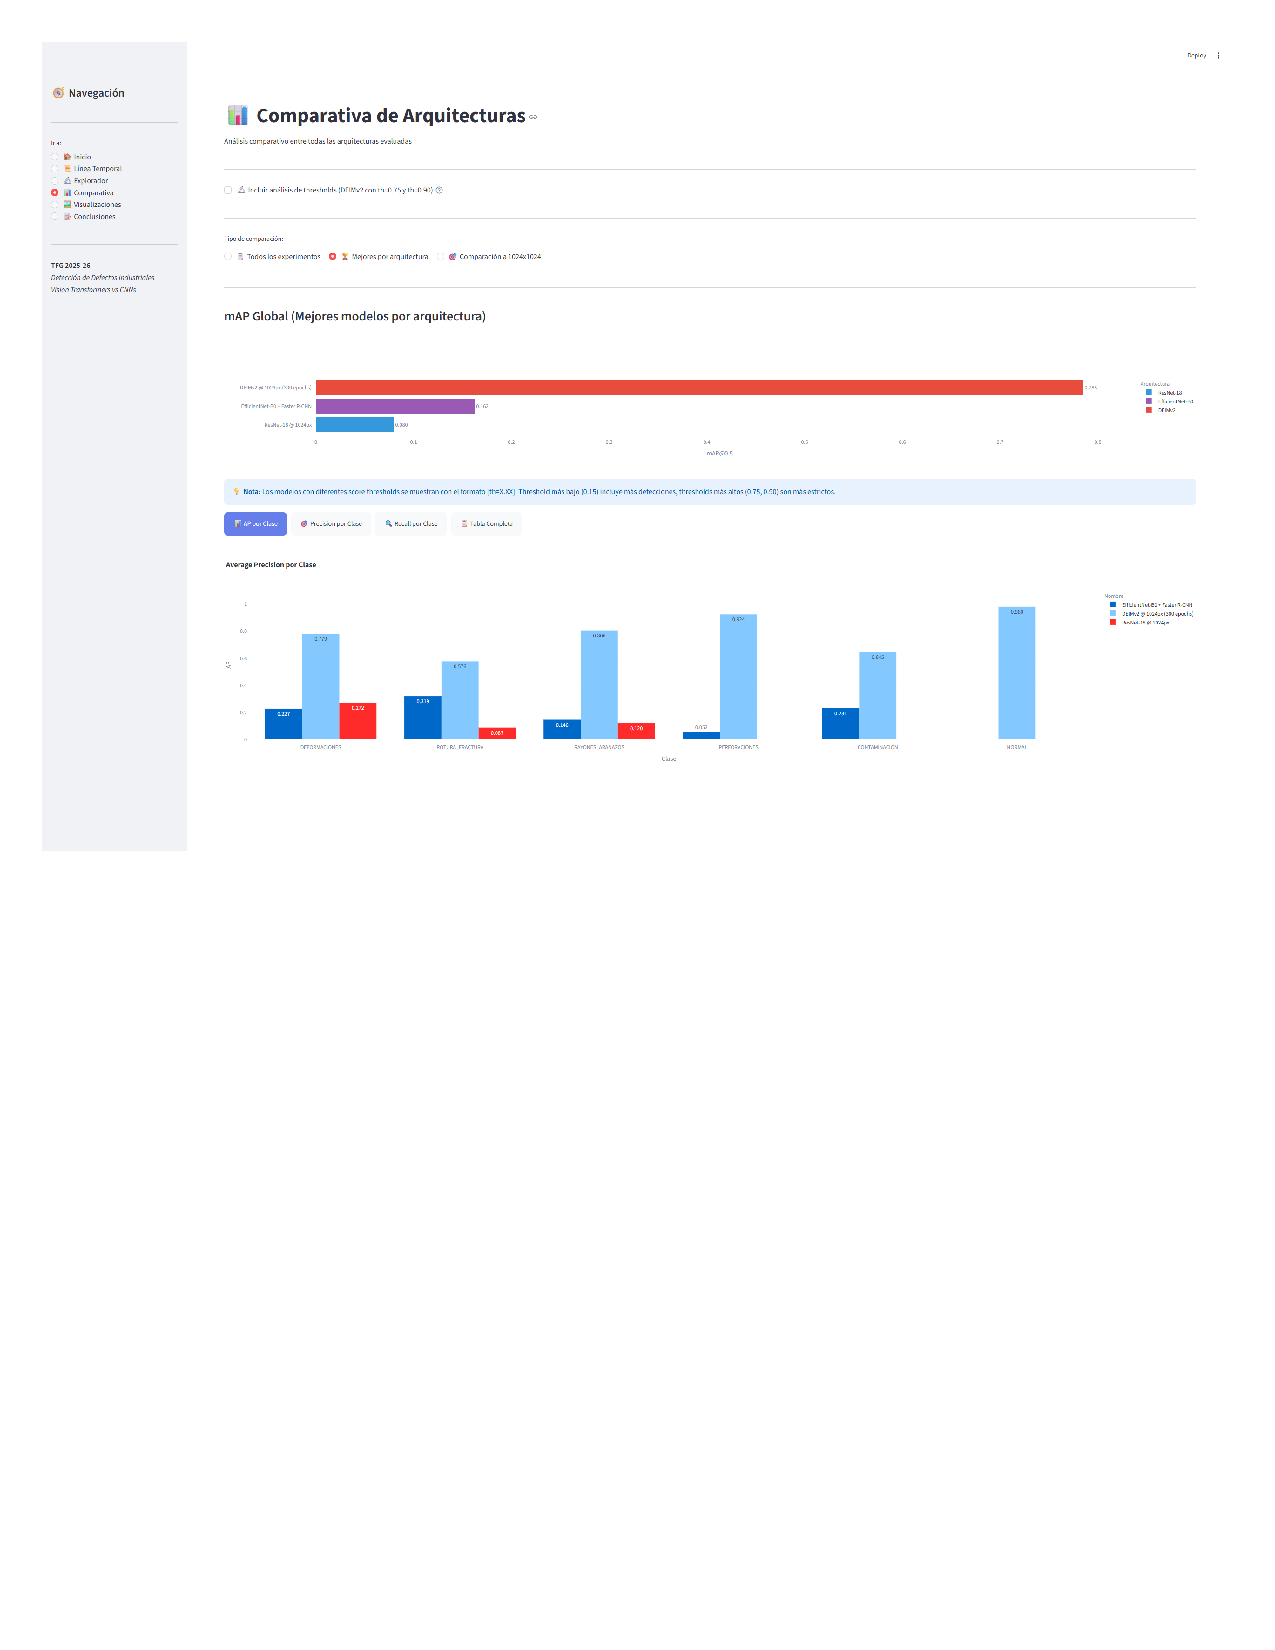
\includegraphics[width=0.95\textwidth]{fig/capturas-pantalla-herramienta-visualizacion/captura-vista-comparativa.pdf}
\caption{Vista Comparativa para el contraste cuantitativo entre arquitecturas a partir de indicadores agregados.}
\label{fig:anexo_cap_comparativa}
\end{figure}

\begin{figure}[htbp]
\centering
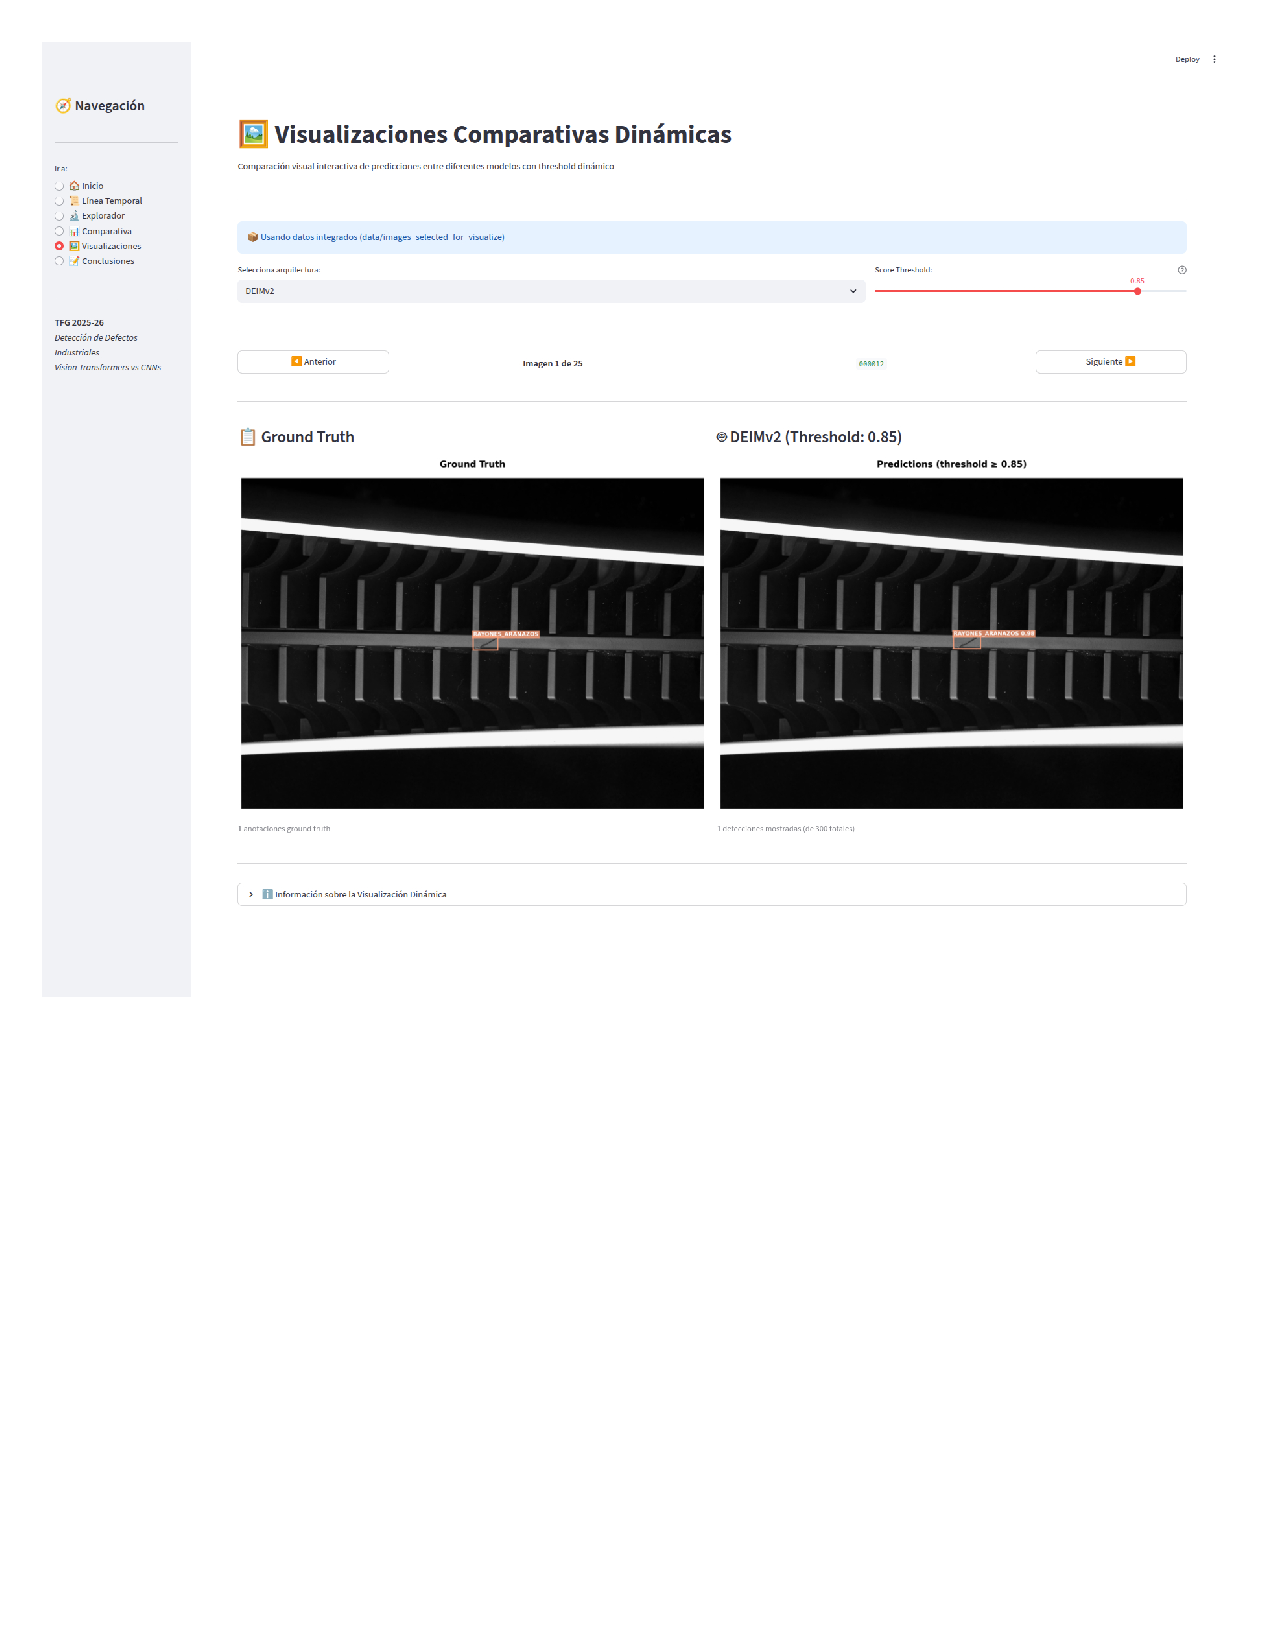
\includegraphics[width=0.95\textwidth]{fig/capturas-pantalla-herramienta-visualizacion/captura-vista-visualizaciones-predicciones.pdf}
\caption{Vista Visualizaciones para la inspección cualitativa (\textit{ground truth} frente a predicción) con ajuste de threshold.}
\label{fig:anexo_cap_visualizaciones}
\end{figure}

\FloatBarrier
